\section{Kinematics of Supersymmetric Events}
\label{sec:kinematic}

The production of supersymmetric particles at hadrcon colliders can generically be
described as
\begin{itemize}
\item pair production of heavy states (such as a $\PSg$ or a $\PSq$);
\item decay to of the heavy particle into a set of final state
  particles consisting of a \emph{visible} subset and an
  \emph{invisible} subset (usually including the $\chiz_1$).
\end{itemize}

For the purposes of this discussion it is useful to consider the
explicit example of squark pair production shown in Fig.~\ref{fig:T2}.
\begin{figure*}[thb!]
\centering
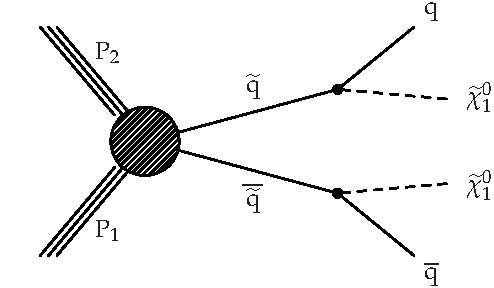
\includegraphics[width=0.49\textwidth]{figs/theory/T2.pdf}
\caption{Diagram featuring squark pair production.\label{fig:T2}}
\end{figure*}

The razor variables \MR and  \Rtwo are motivated by the generic process of the pair production of two
heavy particles (e.g., squarks or gluinos), each decaying to an
undetected particle (the stable, weakly interacting LSP $\chiz_1$)
plus visible particles. The LSP is assumed to escape without
detection, leading to an imbalance $\ptvecmiss$ in the momentum
perpendicular to the beam axis. Each event is treated as a dijet-like event
and the four-momenta of the two jets are used to compute \MR and $\MRT$, defined as
\begin{align}
 \label{eq:MRstar}
 \MR &\equiv
 \sqrt{
(\abs{\vec{p}^{j_{1}}}+\abs{\vec{p}^{j_{2}}})^2 -({p}^{j_1}_z+{p}^{j_2}_z)^2},\\
\MRT &\equiv \sqrt{ \frac{\ETm(\pt^{j_1}+\pt^{j_2}) -
\ptvecmiss \cdot
 (\ptvec^{\,j_1}+\ptvec^{\,j_2}) }{2}},
\end{align}
where $\vec{p}_{j_i}$, $\ptvec^{\,j_i}$, and
$p^{j_i}_z$ are the momentum of the $i$th jet, its
transverse component with respect to the beam axis, and its
longitudinal component, respectively, with $\ETm$ the magnitude of $\ptvecmiss$. While
$\MRT$ quantifies the transverse momentum imbalance,
$\MR$ estimates the mass scale of new-physics particle
production in the event. The razor dimensionless ratio is defined as
\begin{equation}
\R \equiv \frac{\MRT}{\MR}.
\end{equation}

\begin{figure*}[thb!]
\centering
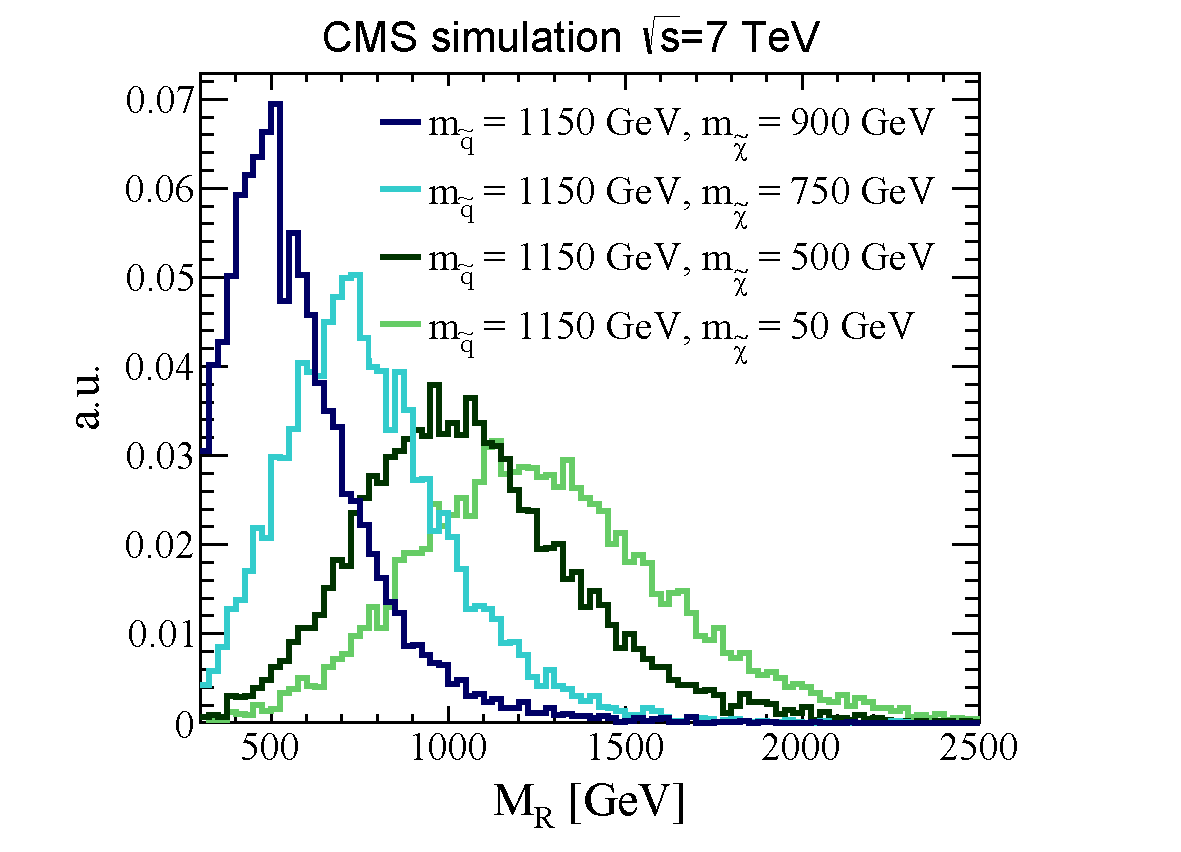
\includegraphics[width=0.49\textwidth]{figs/theory/MR_T2_pheno.pdf}
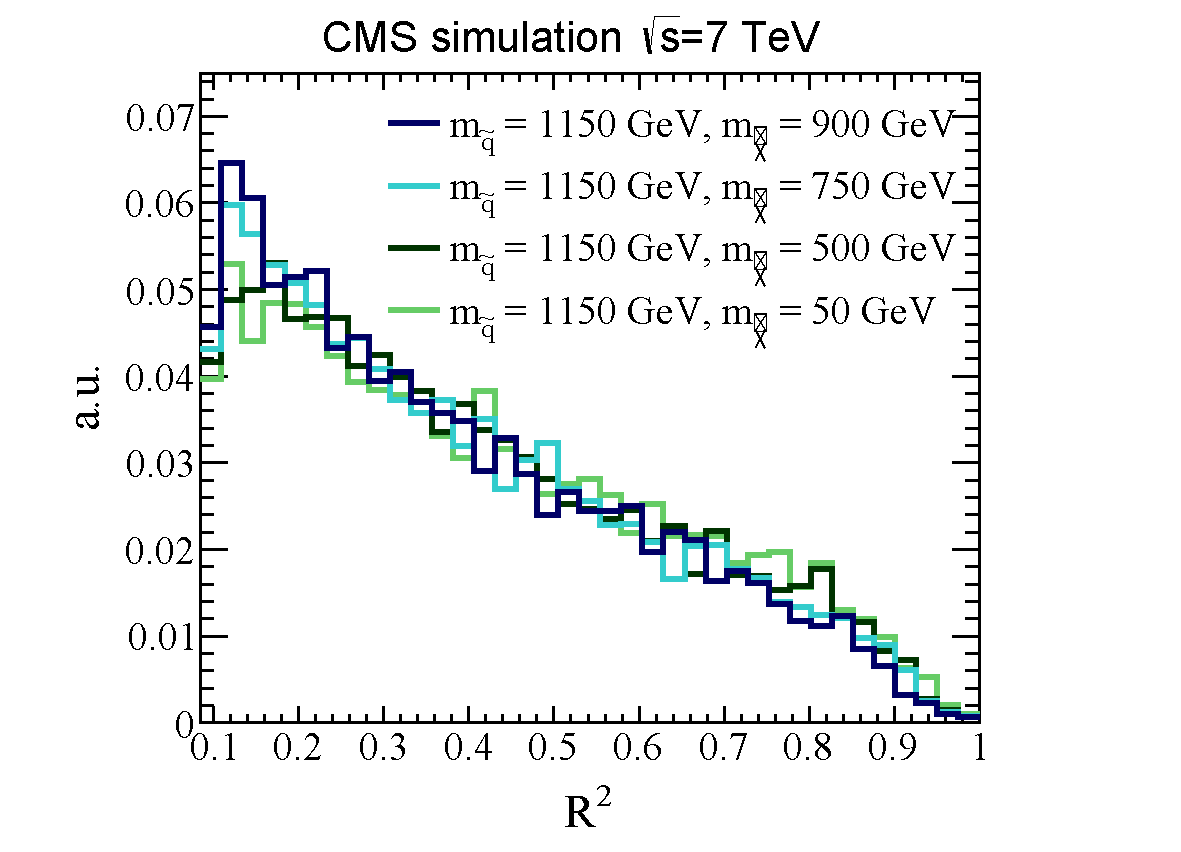
\includegraphics[width=0.49\textwidth]{figs/theory/RSQ_T2_pheno.pdf}\\
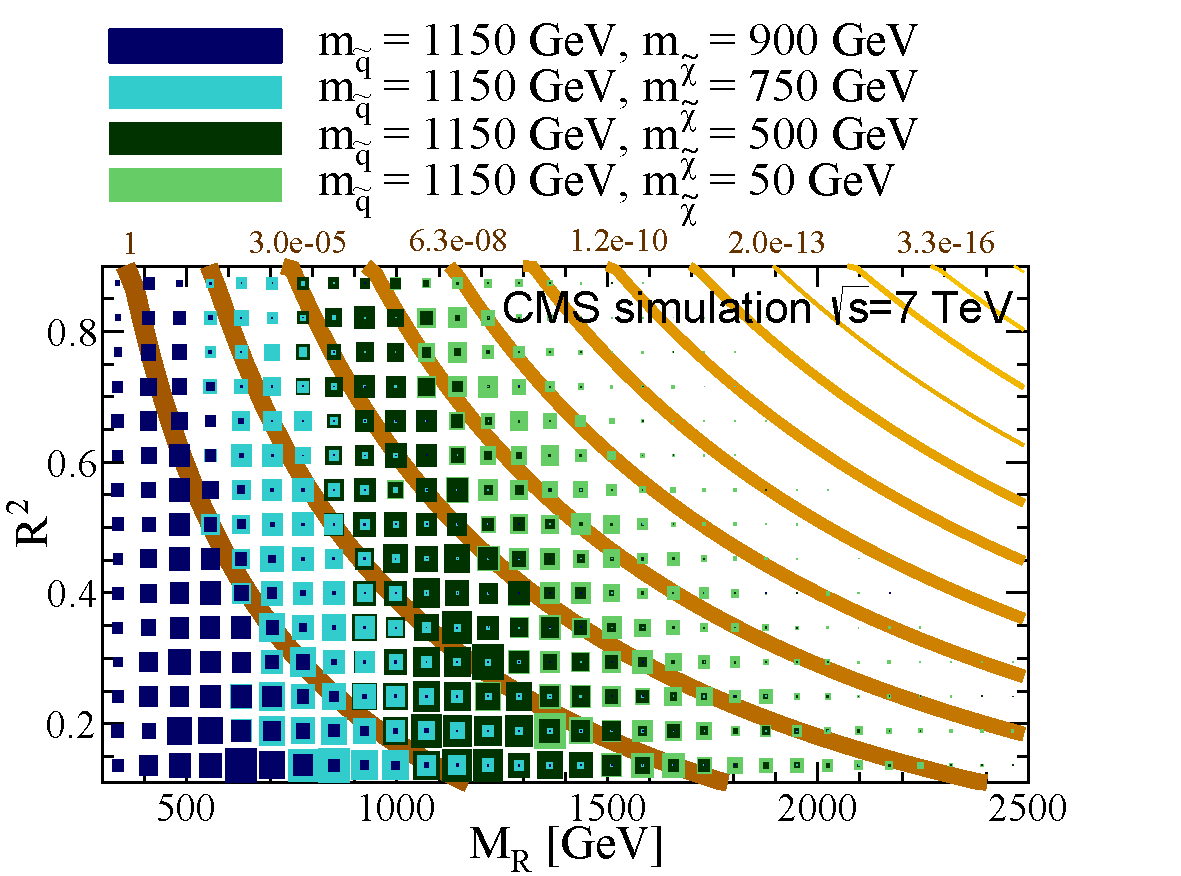
\includegraphics[width=0.49\textwidth]{figs/theory/MR_T2_R2_pheno.pdf}
\caption{Distribution of \Rtwo and \MR for different squark and LSP masses.\label{fig:T2RsqMR}}
\end{figure*}

\textbf{NEED TO EXPAND ON KINEMATICS A LOT}